% Celé zařízení je rozděleno na základní jednotku a~případné moduly, které zajistí nové herní možnosti.
% Například může jít o~připojení úložného prostoru nebo zvukového modulu, který poskytne jak plnohodnotný zvukový výstup tak vstup.

% \subsection{uživatelské požadavky}
Uživatelským požadavkem je statické zařízení sloužící jako herní stanoviště.
Vyžaduje tedy mobilitu, ale jen v~rámci transportu na místo hry a~zpět, nikoliv v~rámci samotné hry.
Z~toho plynou požadavky na velikost výsledného zařízení.

Zařízení bude mít dva světelné kruhy složené z~šedesáti inteligentních RGB LED.
Číslo šedesát jsme zvolili proto, protože se jedná o~dostatečně jemné dělení, aby se daly dělat plynulé efekty.
Zároveň jde o~číslo, které koresponduje s~hodinovým ciferníkem nebo stupnicí na kompasu.
Jeden z~kruhů bude radiální a~druhý axiální.
Axiální je na horní straně zařízení a~slouží primárně jako odezva pro hráče na malou vzdálenost, např. při zadávání hesla.
Radiální kruh je pak také v~horní části zařízení a~slouží naopak pro signalizaci na delší vzdálenost, takový maják.

Uvnitř axiálního světelného kruhu se bude nacházet tzv. tlaková plocha.
Jedná se o~ovládací prvek podobný dotykové ploše, s~tím rozdílem, že je schopen měřit i~sílu, která na něj působí.

Aby bylo stanoviště reálně použitelné při hře, musí celou hru vydržet na baterii.
Není ojedinělé, aby měla outdoorová hra čtyři až pět hodin bez přestávky.
Plus je nutná časová rezerva a~čas na nastavování.
Pochopitelně je čas, který zařízení zvládne běžet z~baterie, silně závisí na činnosti, ale nebylo by zrovna ideální, kdyby byla baterka, výrazně omezujícím faktorem.
Výdrž na jedno nabití by tedy měla být alespoň pět hodin.

Vzhledem k~plánu připojovat moduly je nutné vyřešit, jak se to bude dělat.
Bylo by ideální, kdyby si mohl uživatel říct co bude hrát za hru a~podle toho si sám připojil moduly, které potřebuje.
Tomuto určitě nechceme bránit, ale přímo to podporovat nese řadu problémů, jak ze strany konektoru a~mechaniky, tak ze strany softwaru.
Konektor by totiž musel být ideálně beznástrojově rozpojitelný a~opětovně spojitelný a~přitom dostatečně pevný, aby se zařízení mechanicky chovalo jako jeden celek.
Takový konektor je ale poměrně složité udělat, tak aby byl spolehlivý, a~tak jde v~tuto chvíli spíš o~hudbu budoucnosti.
Ze softwarového pohledu jde pak o~problém jak detekovat konkrétní modul a~hlavně o~otázku jak se chovat k~modulům, které jsou potenciálně záměnné.
Dejme tomu, že máme modul klávesnici a~modul dvířka.
Dvířka jsou původně navržena primárně jako úložný prostor, díky detekci zavření je lze ale použít i~jako velmi pohodlná tlačítka a~v některých hrách se proto používají jen jako tlačítka.
Potenciální modul klávesnice je ovšem jen suma tlačítek.
Při vytváření konkrétní hry na míru modulům, které herní návrhář má zrovna k~dispozici, je tento problém nepodstatný, protože sám návrhář rozhodne, co má jak být.
Ale ve chvíli, kdy jde o~hru navrženou pro jinou kombinaci modulů, nastává problém jak rozhodnout, zda se dají dvířka použít místo klávesnice nebo ne.
Abychom se všem těmto problémům alespoň prozatím vyhnuli, rozhodli jsme, že doplnění či výměna modulu, půjde jen při servisním zásahu.
Problém záměny modulů pak budeme řešit tím, že každá hra bude napsaná jen pro konkrétní sadu modulů.

Některé hry vyžadují tak velké herní území, že by na komunikaci mezi stanovištěmi už nestačila WiFi ani Bluetooth, které AHS jinak využívá ke komunikaci.  
Proto bude mít AHS možnost připojení k~mobilní síti a~tedy připojení k~internetu.
Tím se rozšíří dosah AHS všude, kde je mobilní pokrytí a~také přibude další metoda jak se stanovištěm komunikovat.
V~rámci tohoto komunikačního modulu bude možné používat navíc i~GNSS \footnote{Global Navigation Satellite System}.
Vzhledem k~faktu, že se přece jen nejedná o~systém, který by využila většina her a~zároveň je poměrně drahý, došli jsme k~rozhodnutí mít jej jen jako doplnitelný modul.
Protože se jedná o~modul, který zprostředkovává komunikaci se světem, je pravděpodobné, že bude potřebovat převádět výrazně větší množství dat než běžný modul.
Primárně z~tohoto důvodu je tento modul připojen na samostatném konektoru.
Potřebné antény budou už v~základním zařízení, ale samotný modul spadá do doplňkové výbavy.

V~řadě případů je užitečné mít možnost zvukové zpětné vazby.
Ideální by bylo moci přehrávat libovolnou nahrávku, většinou ale stačí jednoduchý tón, řekněme jako potvrzení zadaného hesla.
Možnost přehrávat plnohodnotnou nahrávku proto odsouváme jako možný doplňkový modul a~v základní jednotce pro jednoduchost postačí piezoměnič.

Z~požadavků nám vyplynulo zařízení, jehož vzhled je nastíněn na obrázku \ref{fig:AHS-nacrt}.
\begin{figure}
    \centering
    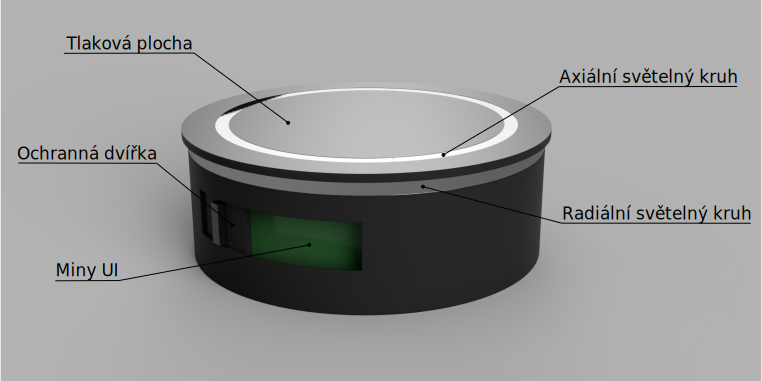
\includegraphics[width=\textwidth]{text/PraktickaCast/img/AHS-nacrt.png}
    \caption{Návrh vzhledu zařízení}
    \label{fig:AHS-nacrt}
\end{figure}

% \begin{itemize}
%     \item Dva LED kruhy jeden radiální na horní straně zařízení a~jeden axiální v~horní části zařízení
%     \item Tlaková plocha
%     \item Výdrž na baterii alespoň pět hodin aby bylo možné organizovat čtyřhodinovou hru s~rezervou na nastavování atd.
%     \item Servisně snadné připojený komunikační/GPS modul uvnitř zařízení
%     \item Servisně snadné připojená dvířka a~jiné moduly vně základního zařízení
%     \item Základní zvuková odezva
% \end{itemize}

\section{Struktura elektroniky základní jednotky}

Elektronika je rozdělena na tři samostatné PCB.
Jde o~hlavní desku, na které je většina elektroniky, o~desku s~hlavním uživatelským rozhraním (LED deska) a~o~obslužnou desku s~minimalistickým uživatelským rozhraním pro neherní obsluhu (Mini UI).

\subsection{LED deska}
Na LED desce se nacházejí oba světelné kruhy a~elektronika pro snímání tlakové plochy, tedy LDC1x14 \cite{LDC1614} a~jeho snímací cívky.
Právě snímaní tlakové plochy je jeden z~podstatných důvodů oddělení této elektroniky na samostatnou desku, zabere totiž docela dost prostoru.

\begin{itemize}
    \item Axiální LED kruh z~60 RGB LED WS2812
    \item Radiální LED kruh z~60 RGB LED WS2812
    \item LDC1614 nebo LDC1314 se čtyřmi snímacími cívkami pro snímání tlakové plochy
    \item konektor na propojení s~hlavní deskou
\end{itemize}

\subsection{Mini UI}
Kvůli aktuální představě mechanické konstrukce není úplně dobře možné mít toto minimalistické uživatelské rozhraní na hlavní desce.
Proto jsme se rozhodli jej vyseparovat na samostatnou destičku, na které bude jen pár tlačítek a~dvě signalizační LED.

\begin{itemize}
    \item RESET tlačítka
    \item BOOT tlačítka
    \item zapínací tlačítko
    \item dvě uživatelská tlačítka 
    \item dvě uživatelské ledky
\end{itemize}

\subsection{Hlavní deska}
Na hlavní desce je většina systému základního zařízení.

Řídící mikrokontroler AHS je ESP32S3 (výběr viz \ref{subs:vyberMikrokontroleru}).

Zdroj AHS je tvořen dvěma LiIon články 18650 v~paralelním uspořádání.
Paralelní uspořádání jsme zvolili, aby nebylo nutné řešit balancování článků.

Aby nebylo možné softwarově baterii podvybít, má AHS ochranu podvybitím, která celé zařízení vypne v~případě, že dojde k~vybití baterie pod 2.8V.
Pochopitelně software by měl vybitou baterii zaznamenat mnohem dřív a~chovat se podle toho, např. neumožnit spustit hru s~baterií při napětí 3.0V.

Na hlavní desce je i~nabíjecí elektronika.
Navíc, aby se minimalizoval čas nabíjení, zařízení podporuje standard Power Delivery a~to až do napětí 21V.

Protože různé periferie vyžadují různá napájecí a~komunikační napětí, jsou na hlavní desce hned čtyři napájecí větve.
\begin{itemize}
    \item VCC, napětí baterie sloužící jako zdroj pro ostatní napájecí větve a~pro napájení komunikačního modulu. 
    \item Napětí \(3.3\-[V]\) na napájení logické části celého základního zařízení.
    \item Napětí \(5.0\-[V]\) pro LED desku a~externí moduly
    \item Napětí \(1.8\-[V]\) pro napájení napěťových převodníků sloužících na komunikaci s~komunikačním modulem 
\end{itemize}
Napětí větví \(3.3\-[V]\) a~\(1.8\-[V]\) je tvořeno pomocí LDO.
Na vytvoření pěti voltové větve je ale potřeba spínaný zdroj a~to primárně ze dvou důvodů.
Za prvé protože napětí baterie, ze které se tato větev napájí, má nižší napětí a~je jej tedy třeba vyspínat na napětí vyšší.
Za druhé tento zdroj poskytuje do systému mnohem větší proudy než druhé dvě větve a~bylo by tedy vhodné ho použít i~v případě použití sériového řazení článků.

Na hlavní desce je také řada konektorů sloužící pro připojení ostatních systémů.
Jde o~konektory na:
\begin{itemize}
    \item propojení s~LED deskou                                            % samostatný objekt
    \item připojení MiniUI                                                  % samostatný objekt
    \item komunikační modul (M2 Konektor umožňuje použít různé moduly)      % externě definovaný objekt
    \item externí moduly                                                    % samostatný objekt
    \item USB-C (nabíjení a~programování AHS)                               % externě definovaný objekt
    \item programátor                                                       % samostatný objekt
\end{itemize}
Do konektorů by se asi dal zařadit i~držák na dva LiIon články 18650.

Za zmínku také stojí přítomnost piezoměniče pro jednoduchou zvukovou odezvu. 

\subsection{Výběr mikrokontroleru \label{subs:vyberMikrokontroleru}}
Požadavky na mikrokontroler jsou:
\begin{itemize}
    \item WiFi
    \item Bluetooth
    \item alespoň 3~UARTy
    \item alespoň 30 GPIO pinů
    \item I2C
    \item dostatečný výpočetní výkon pro hladký chod interpretru JavaScriptu nebo Pythonu
\end{itemize}

Dostupné možnosti jsou:
\begin{itemize}
    \item ESP32                 \cite{ESP32}
    \item ESP32-S3              \cite{ESP32S3}
    \item ESP32-C6              \cite{ESP32C6}
    \item PIC32MZ-W1            \cite{PIC32MZ}
\end{itemize}
Při procházení stránek výrobců jsme nenašli jiný mikrokontroler, který by splňoval všechny požadavky \cite{NordicWiFi}.
Většina mikrokontrolerů s~integrovaným bezdrátovým rozhraním nemá WiFi a~Bluetooth dohromady a~ty co mají, mají zase nedostatek GPIO pinů.
Například nRF7000 \cite{nRF7000} jich má jen 13, RTL8710 17 \cite{RTL8710}, RTL8721 \cite{RTL8721DM} také 17 a~STM32WB55 \cite{STM32WB55} nebo MSP430BT5190 \cite{MSP430BT5190}, zase nemají Wi-Fi.

ESP32-S3 je nástupce ESP32, má vyšší výpočetní výkon, rychlejší paměť a~více pinů.
Oproti ESP32 chybí verzi S3 některé periferie jako například DAC, ty však v~naší aplikaci nevyužijeme a~ESP32 tak můžeme z~výběru vyřadit.
Abychom nemuseli řešit anténu pro WiFi a~Bluetooth, je výhodné použít modul, který ji má integrovanou.
Takový modul existuje pro všechny čtyři zmíněné mikrokontrolery \cite{ESP32-WROOM}\cite{ESP32S3-WROOM}\cite{ESP32C6-WROOM}\cite{WFI32E01PC}, které navíc přidávají třeba flash paměť.
Protože tyto moduly interně používají některé piny, např. všechny tři ESP32 mají interně připojenou flash přes SPI, zmenší se tím počet použitelných GPIO pinů.
Ztráta pinu nám z~výběru vyřadí ESP32-C6, a~kdybychom ho už nevyřadili, vyřadila by i~ESP32.

Výpočetní výkon se porovnává poněkud složitěji a~to proto, že se nejedná tak úplně o~jeden parametr.
Každopádně PIC32MZ-W1 má jedno jádro procesoru DS60001192, který může běžet až na \(200\-[MHz]\)\cite{PIC32MZ}, jinak je ale obtížné o~něm něco bližšího zjistit.
ESP32-S3 má vedle toho dvě jádra procesoru Tensilica Xtensa LX7, která mohou běžet až na \(240\-[MHz]\) \cite{ESP32S3} a~máme na něm vyzkoušený interpreter JavaScriptu, Jaculus \cite{Jaculus}.

Rozhodli jsme se pro ESP32-S3 z~několika důvodů, hlavně proto že s~rodinou mikrokontrolerů ESP32 máme dlouholeté zkušenosti.
Další důvod vyplývá ze skutečnosti, že elektroniku vyrábíme u~firmy JLCPCB.
JLCPCB sice má WFI32 v~nabídce, ale ne na skladě \cite{JSC-WFI32}, zatím co ESP32-S3 mají aktuálně dostupných dokonce 19 variant \cite{JSC-ESP32-S3}.
Navíc je WFI32 za \(13.65\-\$\) zhruba třikrát dražší než ESP32-S3 za cenu okolo \(4\-\$\) \cite{JSC-WFI32}\cite{JSC-ESP32-S3}.

\subsection{Propojení hlavní desky a~LED desky}
Mezi hlavní deskou a~LED deskou je třeba převést napájení a~několik signálů.
LED deska vyžaduje na konektoru přítomnost dvou napájecích větví \(5\-[V]\) pro světelné kruhy a~\(3.3\-[v]\) pro snímání tlakové plochy.
Protože do LEDek může téct proud až 5A a~může být zároveň i~docela rychle spínaný, považujeme za rozumné oddělit napájecím větvím zem.
Oddělení je tedy provedeno už na konektoru hlavní desky.

Na samotné propojení jsme se rozhodli použít FFC kabel s~roztečí \(0.5\-[mm]\).
Jedním vodičem takovéhoto kabelu lze vést proud maximálně \(0.4\-[A]\) \cite{FFC-konektor}.
Protože ale potřebujeme dodat proud až 5A, použijeme 13 vodičů vedle sebe jakožto nejmenší počet, který přenese požadovaný proud v~rámci daných mezí.

Mimo napájení je tímto propojením veden i~signál s~daty pro světelné kruhy a~I2C sběrnice s~interruptem pro připojení čipu LDC1614 \cite{LDC1614}.

Vzhledem k~počtu potřebných vodičů (konkrétně 32) jsme se rozhodli použít velmi běžný FFC konektor se 40 kontakty, s~tím že zbylé kontakty se mohou hodit v~budoucnu.

\subsection{Modulový konektor}
Modulovým konektorem je vedeno \(5\-[V]\) jako napájení pro moduly a~UART s~interruptem pro komunikaci.
Nad volbou komunikační sběrnice jsme strávili poměrně dost času přemýšlením.
Původně jsme uvažovali o~využití RS485 jakožto odolné sběrnice, u~které by v~případě potřeby nemusel být problém ani delší kabel.
RS485 má ale nevýhodu v~tom, že potřebuje dodatečný hardware, kterému bychom se hlavně na modulech rádi vyhnuli.
Stejný problém nastal u~CANu i~USB, které by navíc mělo výhodu kompatibility s~velkým množstvím hotových zařízení.

V~první úvaze o~UARTu jsme jej nejprve zavrhli kvůli potenciální náročnosti na přeposílání dat mezi moduly.
Při standardním použití bychom totiž moduly řadili za sebe.
Prvnímu modulu by tak chodili data pro všechny ostatní moduly a~musel by je přeposílat dál, což by stálo nezanedbatelné množství procesorového času.
V~jisté chvíli jsme ale narazili na nestandardní komunikaci pomocí UARTu implementované v~projektu Servio \cite{Servio}.
Tato implementace používá UART jako sběrnici.
Namísto standardního použití pro komunikace jeden s~jedním tak může komunikovat jeden s~více.
Na tomto řešení je výhodné, že nevyžaduje žádný dodatečný hardware a~prakticky každý dnešní mikrokontroler je možné k~této sběrnici velmi snadno připojit.
Ve srovnání s~RS485 je sice mnohem méně odolná proti rušení, ale uvnitř zařízení nebude linka vedena na víc než malé desítky centimetrů.
Komunikace na delším kabelu je pak jednoduše nahraditelná bezdrátovou komunikací a~není tak potřebné, aby to nativně umožňovala tato sběrnice.
Každopádně v~případě potřeby delšího kabelu je možné navrhnout externí modul, který s~této sběrnice velmi jednoduše udělá RS485.
Alternativně by se pro komunikaci na delším kabelu dalo použít USB, které je společně s~nabíjením přivedeno na USB-C.

Všechny moduly jsou tedy připojeny na jeden RX pin AHS.
Proto musí firmware AHS zajistit, aby dva moduly nevysílaly současně.
Aby se zabránilo možným zkratům, jako ochranu má každý modul své piny UARTu připojeny přes rezistor \(180\-[\Omega]\).
Interrupt pin modulů se naopak chová jako open-collector a~na straně hlavního zařízení je na něj tedy připojen pull-up rezistor.
Abychom alespoň trochu zvýšili odolnost linky proti rušení, přidáme na přijímací stranu pull-up rezistor.
Cílem je zvýšení komunikačního proudu, aby se případný proud vyvolaný rušením dal jednodušeji zanedbat.
V~neposlední řadě mají všechny piny na konektoru ESD ochranu.

\newpage
\subsection{Konektor programátor}
Zařízení se dá jednoduše programovat přes USB-C, tento kanál se ale dá softwarově narušit a~pro takové případy je tu konektor na programátor.
Jde o~šest plošek, na které se programátor připojuje pomocí pogo-pinů.
Programátor sice obsahuje jen jednoduchou elektroniku, která by mohla být i~přímo v~elektronice AHS, ale ve většině případů by byla zbytečná.
Ve chvíli, kdy by byla potřeba, je stejně nutná odborná obsluha a~pro tu není problém použít programátor.
\begin{figure}[h]
    \begin{minipage}[l]{0.55\textwidth}
        
        Aby bylo možné zařízení programovat přes dedikovaný programovací konektor, je na konektoru i~\(5\-[V]\) napájení.
        To ale způsobuje problém ve chvíli, kdy je zařízení zároveň připojeno přes USB-C, protože se v~tu chvíli tyto zdroje zkratují.
        % Proto je na konektoru programátor i~ochrana, která v~případě připojení USB-C odpojí napájení z~programátoru, neboli jedna dioda. %jako vtip který vymyslel gitkopilot super 
        Proto je toto napájení přivedeno přes diodu, která v~případě připojení USB-C odpojí napájení z~programátoru.
        Zapojení konektoru je vidět na obrázku \ref{fig:programator}.
    \end{minipage}
    \hfill
    \begin{minipage}[r]{0.4\textwidth}
        \centering
        \includegraphics[width=\textwidth]{text/TeoretickyUvod/AplikaceHernichZarizeni/img/programator.png}
        \caption{Programovací konektor}
        \label{fig:programator}
    \end{minipage}
    
\end{figure}


\subsection{USB-C}
Jako napájecí a~programovací konektor je použito USB-C.
Díky němu je možné podporovat standard Power Delivery využitý pro zrychlení nabíjení.
Konektor je ale použit i~na pohodlnější programování zařízení, bez potřeby programátoru.

\subsection{Konektor komunikačního modulu}
Pro připojení komunikačního modulu jsme zvolili konektor M2 typ-B jakožto standard pro tyto moduly.
Díky tomuto konektoru můžeme jednoduše připojit různé LTE a~GNSS moduly.




% Na konektor, je z~ESP vyvedeno: 
% -   I2C
% -   celý UART
% -   FUL_CARD_POWER_OFF
% -   RESET
% -   WoWWAN (interrupt)

% a~mimo ESP je na konektoru:
% -   napájení přímo z~baterie
% -   SIM

% Pin-out M2 konektoru z~https://files.waveshare.com/upload/0/02/SIM7600X-M2_Hardware_Design_V1.01.pdf
% ![](img/SIM7600G-H-M.2-PIN.png)


% ## mechanická část
% Základ AHS je mechanicky krátký válec s~tlakovou plochou na horní ploše.
% Kolem tlakové plochu je umístěn axiální světelný kruh a~v horní části válcové plochy je radiální světelný kruh.

% - Tělo minimálně v~prototypu tisknuté
% - Vyzkoušet různé provedení kontaktní plochy
%     - Stejně jako na předchozí verzi FR4 ale tlustší, aby se tolik nekroutila
%     - PCB s~hliníkovým jádrem + zalití do epoxidu nebo jiné dostatečně průsvitné hmoty
% - Konektor externích modulu, USB-C a~mini UI překrýt krytkou (ochrana před bordelem a~náhodným mačkáním na tlačítka) 

% ![](img/dvirka.png)
